\section{ガイド磁場コイル}
ガイド磁場コイルには二つの役割を持っている:

\begin{enumerate}
\item 実験装置全体に渡って中性子の量子化軸を定める
\item 垂直方向に地磁気を無視できる程の大きさの磁場を一様に印加する
\end{enumerate}

特に二つ目の役割は重要であり、磁場の大きさが地磁気に比べて十分大きくないと地磁気によるスピンの反転が起きてしまうことになる。
図\ref{device_fig_guide}はガイド磁場コイルに1Aの電流を流したときの磁場分布シミュレーション結果である。このシミュレーションから得られた$y,z$方向それぞれ$\pm0.04$mの範囲における磁場の不均一性は$y$方向が2.5\% $z$方向が1.6\% 程度に抑えられており、この磁場の一様性は中性子が通過する場所によって干渉条件が大きくずれないことを保証する。
実験ではガイド磁場コイルに5.5Aの電流を流し、ビーム軸上で磁場の強さは約12.8Gとなった。
なお電流を5.5A流すとガイド磁場コイルの温度が60$^\circ$C以上になる部分もあったため、3台の扇風機で空冷しながら実験を行った。

\begin{figure}[H]
\begin{center}
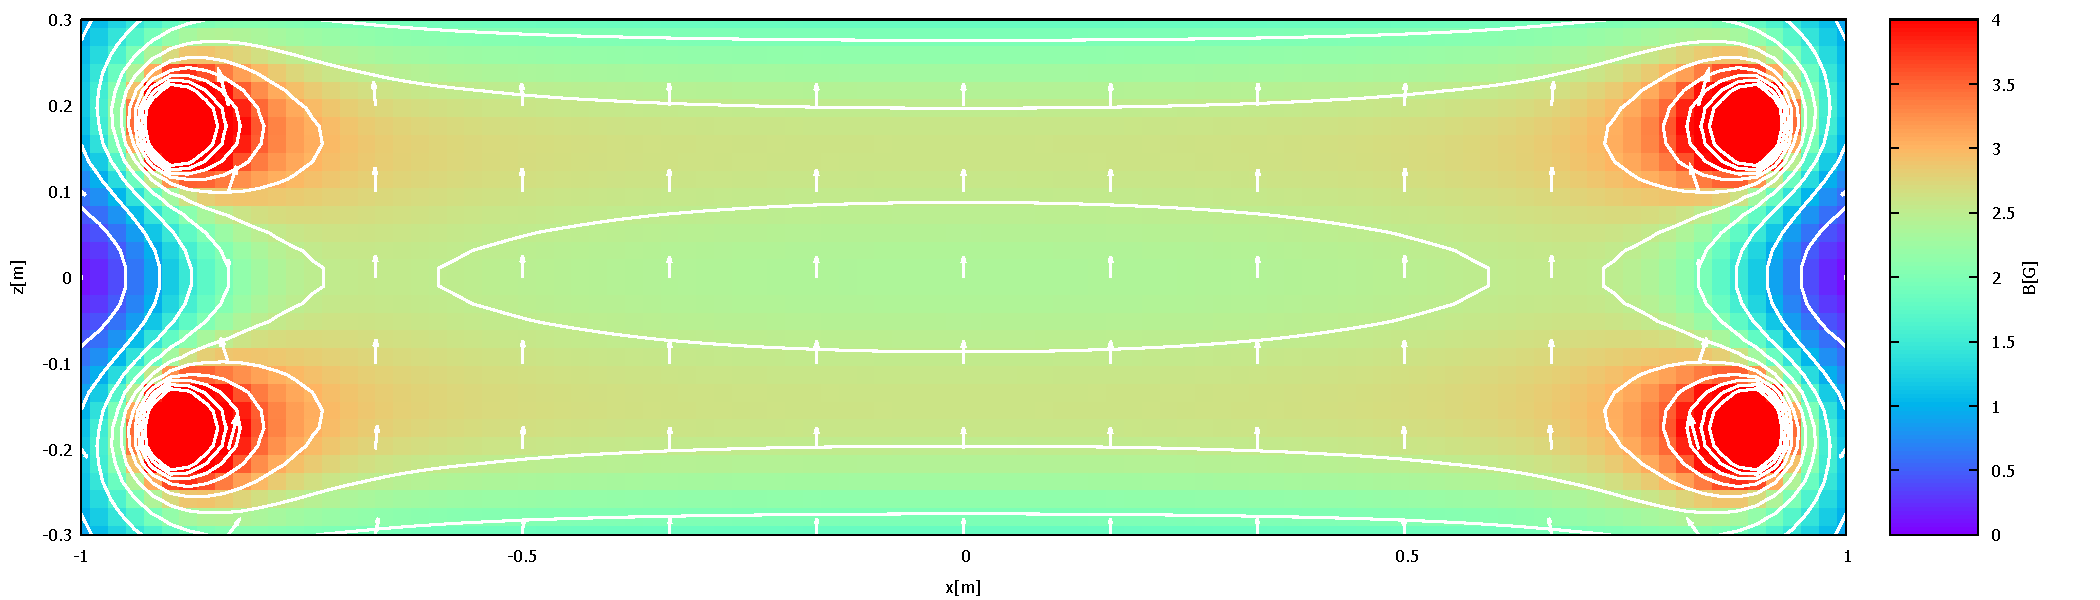
\includegraphics[width=10cm]{device/coil4_image1.pdf}
\subcaption{横から}
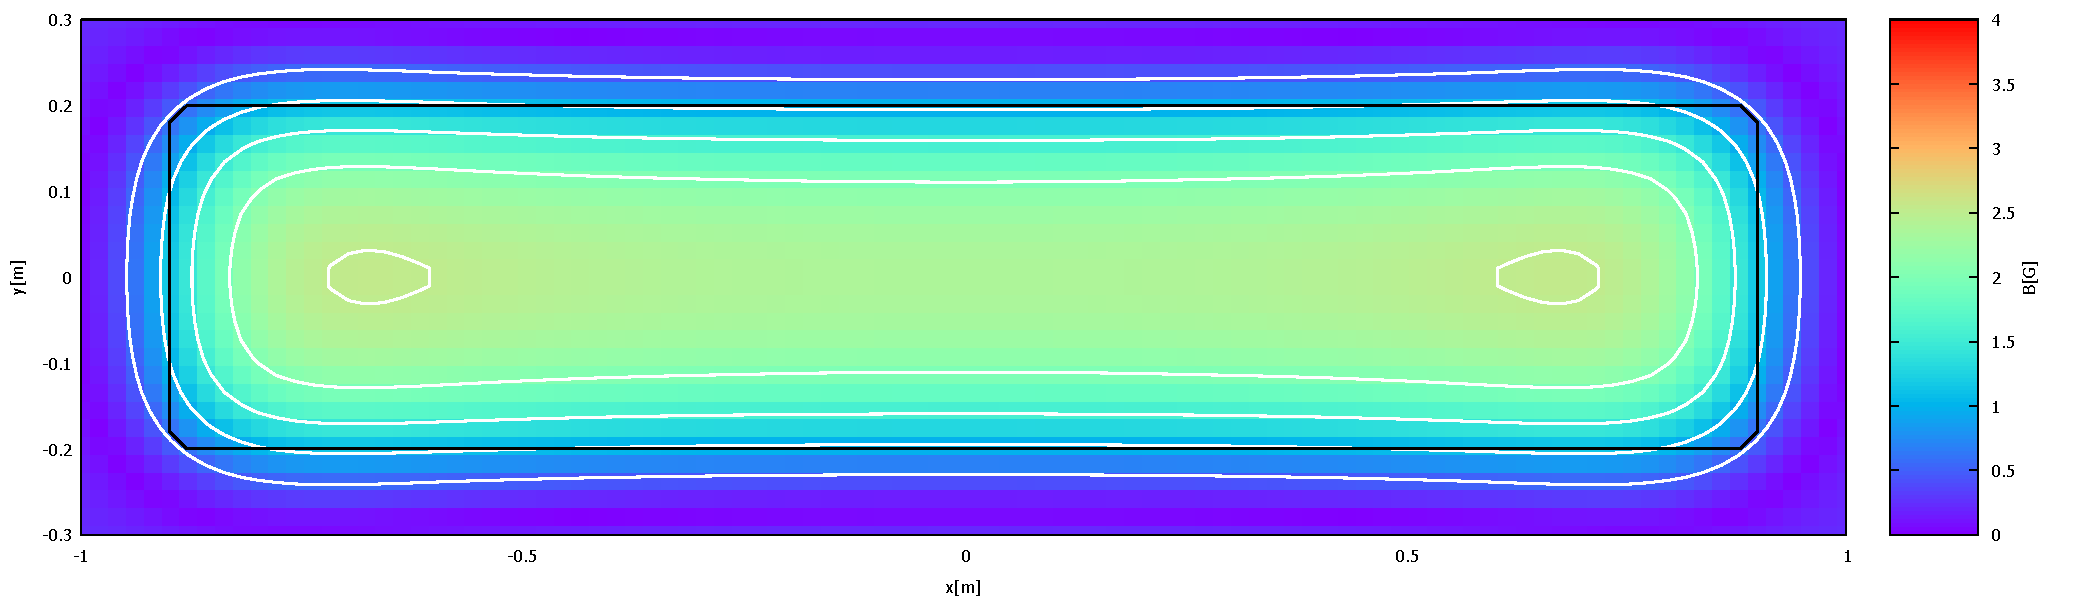
\includegraphics[width=10cm]{device/coil4_image2.pdf}
\subcaption{上から}
\end{center}
\vspace{-5mm}
\caption{ガイド磁場コイルの磁場分布シミュレーション}\label{device_fig_guide}
\vspace{-5mm}
\end{figure}
\begin{figure}[H]
\centering
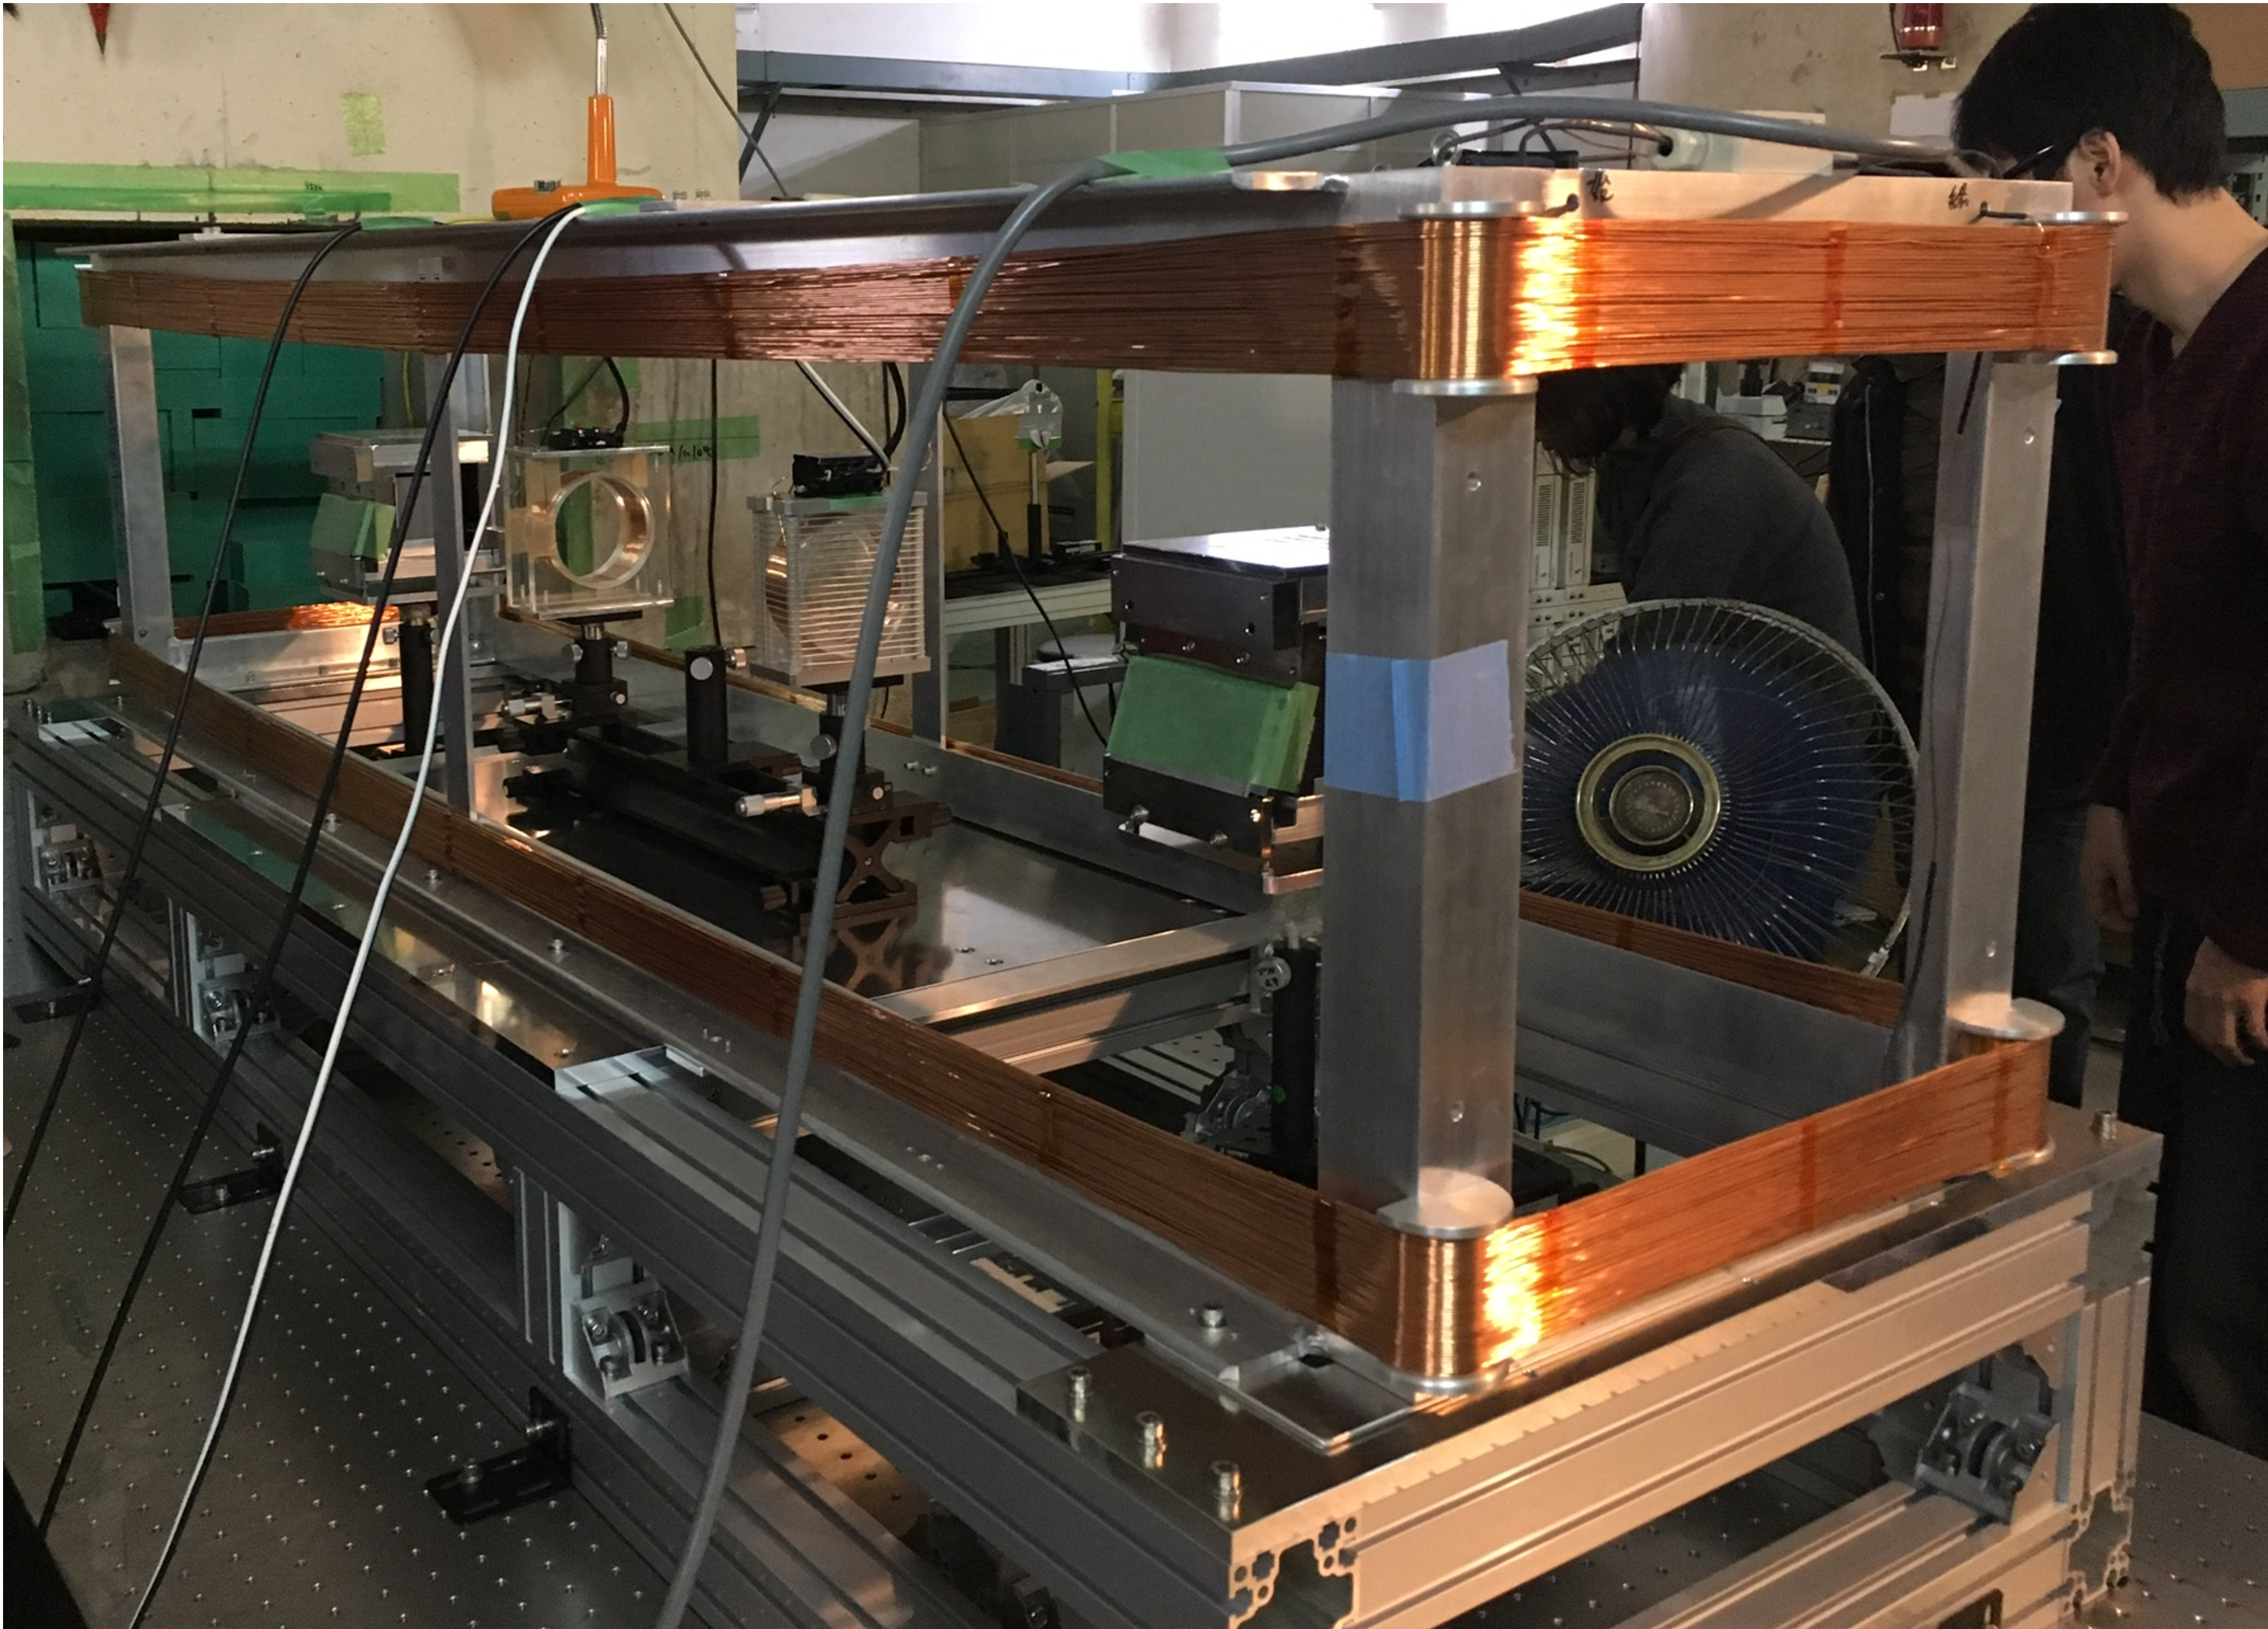
\includegraphics[width=7cm]{device/coilphoto.pdf}
\caption{ガイド磁場コイル}
\vspace{-1cm}
\end{figure}